\section{Methodology}
\label{sec:method}

Our approach to establishing pixel-accurate semantic correspondences is structured into four progressive stages, leveraging the rich internal representations of Visual Foundation Models (VFMs).

\subsection{Phase 1: Training-Free Baseline}
The baseline relies entirely on the frozen latent representations of pre-trained backbones (DINOv2, DINOv3, and SAM) without gradient updates. For a given pair of source and target images, dense feature maps are extracted. To match a specific source keypoint, we compute the cosine similarity between its corresponding feature vector and all patch features in the target image. The predicted match is obtained using a standard, non-differentiable \textit{argmax} operator on the resulting similarity map. To ensure precise alignment, images are resized to a fixed resolution — $518\times518$ for DINOv2 (37 patches of size 14) and $512\times512$ for DINOv3 and SAM (32 patches of size 16). SAM additionally upsamples internally to $1024\times1024$ before encoding; keypoint coordinates are mapped back to the $512\times512$ frame.

\subsection{Phase 2: Light Fine-Tuning}
To improve domain adaptation and correspondence accuracy, we perform supervised fine-tuning by unfreezing only the final layers of the vision encoders, keeping early representation layers frozen. We optimize the network using a Gaussian Cross-Entropy loss. Instead of penalizing all non-exact pixel predictions equally, this loss relaxes the ground truth point into a 2D Gaussian probability distribution, computing the cross-entropy against the predicted softmax probability map. This formulation accounts for the inherent ambiguity in dense matching.

\subsection{Phase 3: Inference Refinement}
The standard \textit{argmax} operation locks predictions to discrete patch centers and is highly sensitive to local noise peaks. To achieve sub-pixel accuracy at inference time, we replace it with the Windowed Soft-Argmax (WSA). As illustrated in Figure~\ref{fig:wsa_pipeline}, WSA first identifies the coarse peak via \textit{argmax}, instantiates a small fixed window (e.g., $5 \times 5$) around this peak, and applies a soft-argmax operation exclusively within this local region. This step is applied solely during evaluation and does not affect the training objective.

\begin{figure}[ht]
    \centering
    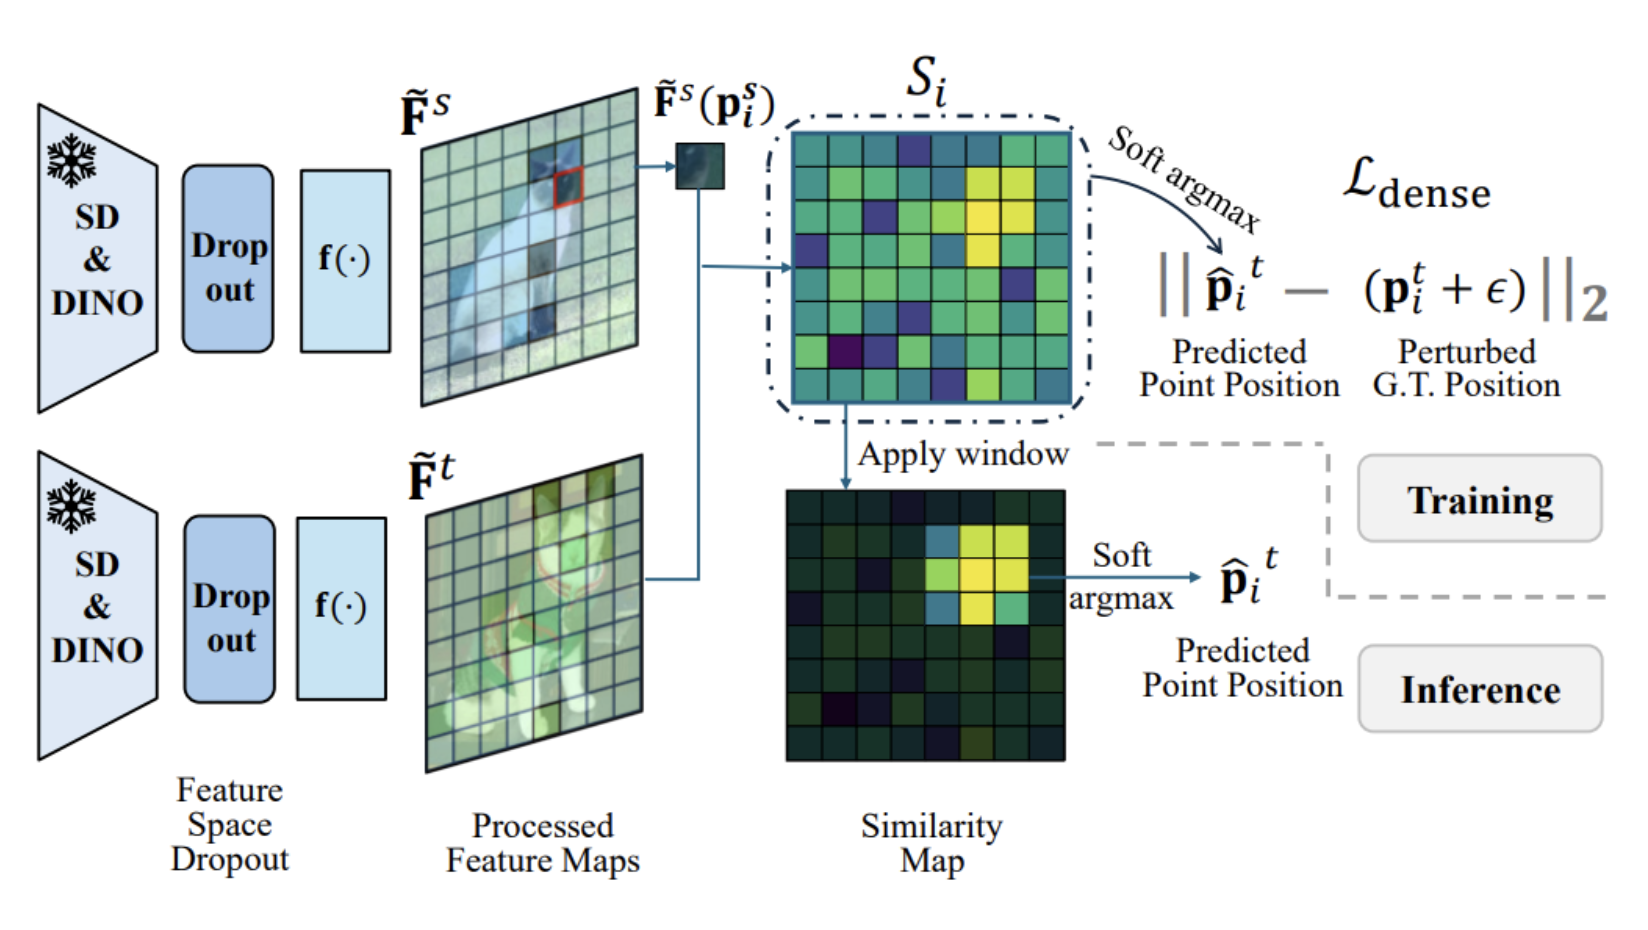
\includegraphics[width=\columnwidth]{img/wsa_pipeline.png}
    \caption{Overview of the dense matching pipeline and Inference Refinement. The similarity map is processed using a Windowed Soft-Argmax to achieve robust, sub-pixel accurate keypoint predictions.}
    \label{fig:wsa_pipeline}
\end{figure}

\subsection{Phase 4: Extensions (Parameter-Efficient Fine-Tuning)}
As an advanced exploration, we implemented a Parameter-Efficient Fine-Tuning (PEFT) strategy using Low-Rank Adaptation (LoRA). Full fine-tuning of massive vision backbones is computationally expensive and memory-intensive. To mitigate this, LoRA freezes the pre-trained model weights and injects trainable rank-decomposition matrices into the network. 

In our implementation, we applied manual LoRA adapters exclusively to the Multilayer Perceptron (MLP) linear layers of the final Transformer blocks. This surgical intervention drastically reduces the number of trainable parameters while giving the model enough flexibility to adapt to the semantic correspondence task on the SPair-71k dataset.